%
% fig-abstandtex
%
% (c) 2025 Prof Dr Andreas Müller
%
\begin{figure}
\centering
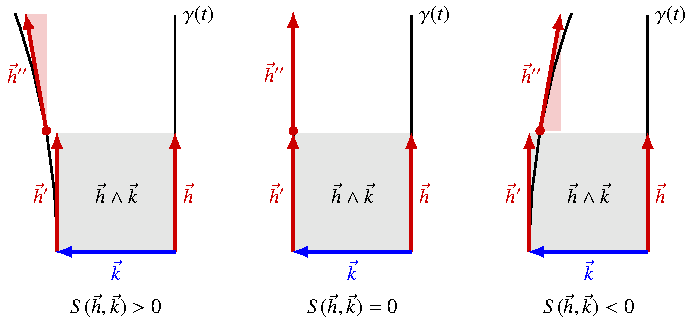
\includegraphics{chapters/110-kruemmung/images/abstand.pdf}
\caption{Schnittkrümmung und der Abstand von Geodäten mit
parallelverschobener Anfangsrichtung, die von infinitesimal
benachbarten Punkten ausgehen.
Bei positiver Schnittkrümmung wird der Abstand grösser, bei negtiver
Schnittkrümmung wird er kleiner.
\label{buch:kruemmung:schnittkruemmung:fig:abstand}}
\end{figure}
